\documentclass[12pt]{article}
\usepackage[utf8]{inputenc}
\usepackage[brazil]{babel}
\usepackage{hyphenat}
\usepackage{graphicx}
\usepackage{amsmath}
\graphicspath{{images/}}
\usepackage{float}
\usepackage{amsmath}

% ---- Capa
\title{%
    Modelagem de Sistemas Dinâmicos\\
    \large Trabalho 4}
\author{Erica da Cunha Ferreira}
\date{Novembro 2020}
\begin{document}
\maketitle
\pagenumbering{gobble}
\vspace{8cm} %5mm vertical space
\begin{center}
    
\includegraphics[width=0.2\textwidth]{logo.png}
\end{center}

%-----Sumário
\newpage
\tableofcontents
\newpage
\pagenumbering{gobble}

%----Pág 1
\cleardoublepage\pagenumbering{arabic}

\section{Introdução}

\quad Este trabalho tem como objetivo analisar o sistema do $Segway$, como um pêndulo invertido de duas rodas. 

\begin{figure}[H] 
    \centering
    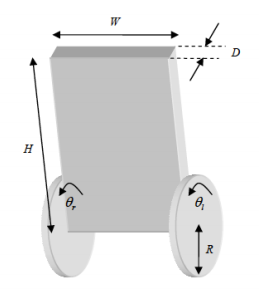
\includegraphics[width=0.4\textwidth]{trab4_fig1.png}
    \caption{Sistema de Pêndulo Invertido}
    \label{fig:mesh1}
\end{figure}

\quad Abaixo temos as vistas lateral e superior do sistema.

\begin{figure}[H] 
    \centering
    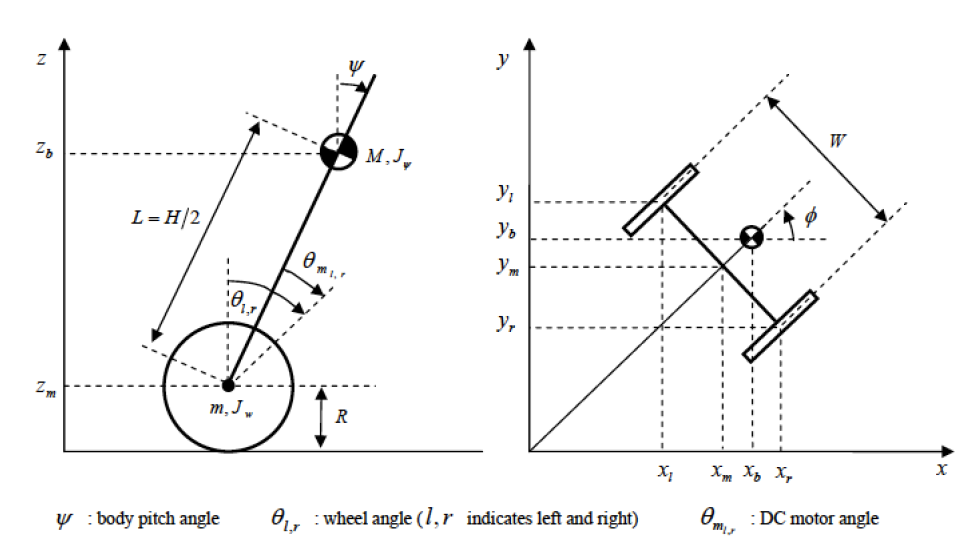
\includegraphics[width=0.9\textwidth]{FIGURA1.png}
    \caption{Visão Lateral e Superior do Sistema}
    \label{fig:mesh4}
\end{figure}

Temos os parâmetros físicos deste sistema que são:

\begin{itemize}
    \item $g = 0.98$ $m/s^2$, gravidade.
    \item $m = 0.03$ $kg$, peso da roda.
    \item $R = 0.04$ $m$, rádio da roda.
    \item $M = 0.6$ $kg$, peso do corpo.
    \item $W = 0.14$ $m$, largura do corpo.
    \item $D = 0.04$ $m$, profundidade do corpo.
    \item $H = 0.144$ $m$, altura do corpo.
    \item $J_m = 10^{-5}$ $kg\cdot m^2$, inércia do motor DC.
    \item $R_m = 6.69$  $\Omega$, resistência do motor DC.
    \item $K_t = K_e = 0.4$, constante de torque e de EMF.
\end{itemize}

\section{Metodologia}

\quad A partir desses dados e da figura dos sistema podemos chegar às seguintes equações:

\begin{equation}
    J_w = \frac{m\cdot R^2}{2}
\end{equation}

\begin{equation}
    L = \frac{H}{2}
\end{equation}

\begin{equation}
    J_y = \frac{M \cdot L^2}{3}
\end{equation}
 
\begin{equation}
    J_o = \frac{M \cdot(W^2 + D^2)}{12}
\end{equation} 

\begin{equation}
    \alpha = \frac{n \cdot K_t}{R_m}
\end{equation}

\begin{equation}
    \beta = \frac{n \cdot K_t \cdot K_b}{R_m} + f_m
\end{equation}

\begin{equation}
    J = \frac{W^2 \cdot (b + f_w)}{2R^2}
\end{equation}

\begin{equation}
    I = \frac{m \cdot W^2}{2} + J_o + \frac{W^2 \cdot (J_w + J_m \cdot n^2)}{2 \cdot R^2}
\end{equation}

\begin{equation}
    K = \frac{W \cdot a}{2R}
\end{equation}

\begin{equation}
    f_w = 0
\end{equation}

\begin{equation}
    n = 1
\end{equation}

\begin{equation}
    F_m = 0.0022
\end{equation}
 
\subsection{Análise de Lagrange}

\quad Ao analisar a \textbf{Figura 2} e ao considerar a direção positiva para o pêndulo no tempo de $t = 0$ $segundos$, chegamos às seguintes expressões do sistema: 

\begin{equation}
    \theta,\phi = \frac{(\theta_1 + \theta_r)\cdot (\theta_r - \theta_i) \cdot R}{2 \cdot W} 
\end{equation}

\begin{equation}
    x_m, y_m,z_m = \int{ \Dot{x}_m dt}, \int {\Dot{y}_m dt}, R
\end{equation}

\begin{equation}
    \Dot{x}_m,\Dot{y}_m = R \cdot \Dot{\theta} \cdot  \cos{\phi}, R \cdot  \Dot{\theta} \cdot \sin{\phi}
\end{equation}

\begin{equation}
    x_l,y_l,z_l = x_m - \frac{W \cdot \sin{\phi}}{2}, y_m + \frac{W \cdot \cos{\phi}}{2} , z_m
\end{equation}

\begin{equation}
    x_r,y_r,z_r = x_m + \frac{W \cdot \sin{\phi}}{2}, y_m - \frac{W \cdot \cos{\phi}}{2}, z_m
\end{equation}

\begin{equation}
    x_b, y_b, z_b = x_m + L \cdot \sin{\Psi} \cdot \cos{\phi},y_m + L \cdot \sin{\Psi} \sin{\phi}, z_m + L \cdot \cos{\Psi}
\end{equation}

\quad Sendo $T_1$  e $T_2$ as energias cinéticas de translação e rotação, respectivamente, e U a energia potencial total do sistema, temos:

\begin{equation}
    T_1 = \frac{m \cdot [(\dot{x}_l^2 + \dot{y}_l^2 + \dot{z}_l^2) + ( \dot{x}_r^2 + \dot{y}_r^2 + \dot{z}_r^2)] + M \cdot [(\dot{x}_b^2 + \dot{y}_b^2 + \dot{z}_b^2)]}{2}
\end{equation}

\begin{equation}
    T_2 = \frac{J_w(\Dot{\theta}_l^2 +\Dot{\theta}_r^2) +J_{\Psi} \dot{{\Psi}}^2 + J_{\phi}\dot{{\phi}}^2+ n^2 J_m[(\dot{\theta}_l - \dot{\phi})^2 + (\dot{\theta}_r - \dot{\Psi})^2]}{2}
\end{equation}

\begin{equation}
    U = mgz_l + mgz_r + Mgz_b
\end{equation}

Partindo do princípio geral do Lagrangiano:

\begin{equation}
    L = T_1 + T_2 - U
\end{equation}

Sendo as nossas variáveis generalizadas:

\begin{equation}
    \lambda = 
    \begin{bmatrix}
    \theta\\
    \Psi \\
    \phi
    \end{bmatrix}
\end{equation}

Então, temos como base as expressões:

\begin{equation}
    \frac{d}{dt}\left(\frac{\partial L}{\partial \Dot{\theta}}\right) - \frac{\partial L}{\partial \theta} = F_{\theta}
\end{equation}

\begin{equation}
    \frac{d}{dt}\left(\frac{\partial L}{\partial \Dot{\Psi}}\right) - \frac{\partial L}{\partial \Psi} = F_{\Psi}
\end{equation}

\begin{equation}
    \frac{d}{dt}\left(\frac{\partial L}{\partial \Dot{\phi}}\right) - \frac{\partial L}{\partial \phi} = F_{\phi}
\end{equation}

Com isso temos que:

\begin{equation}
    [(2m + M) R^2 + 2J_w + 2n^2J_m)]\ddot{\theta} + \left(MLR \cdot \cos{\Psi} - 2n^2J_m\right)\ddot{\Psi} - MLR \Psi 2\sin{\Psi} = F_{\theta}
\end{equation}

\begin{equation}
    (MLP \cdot \cos{\Psi} + 2n^2 J_m) \ddot{\theta} + (ML^2 + J_{\Psi} + 2n^2J_m)\ddot{\Psi} - MgL\sin{\Psi} - ML^2\dot{{\phi}}^2\sin{\Psi}\cos{\Psi} = F_{\Psi}
\end{equation}

\begin{equation}
    \left (\frac{m \cdot W^2 J_{\phi}}{2} + \frac{W^2 \cdot (J_w + n^2J_m)}{2R^2} + ML^2{\sin^2{\Psi}} \right)\ddot{\theta} + 2\cdot ML^2 \cdot \dot{\phi} \cdot  \dot{\Psi} \cdot  \sin{\Psi} \cdot \cos{\Psi} = F_{\phi} 
\end{equation}

Considerando o torque do motor DC e atrito, temos as seguintes forças generalizadas do sistema:

\begin{equation*}
    F_{\theta}, F_{\Psi},F_{\phi} = F_l + F_r, F_{\Psi}, \frac{W\cdot ( F_r - F_l)}{2 \cdot R} 
\end{equation*}

\begin{equation*}
    F_l = n K_t i_l + f_m(\dot{\Psi} - \dot{\theta_l}) - f_w \dot{\theta_l} 
\end{equation*}

\begin{equation*}
     F_r = n K_t i_r + f_m(\dot{\Psi} - \dot{\theta_l}) - f_w \dot{\theta_r} 
\end{equation*}


\begin{equation*}
     F_{\Psi} = -n K_t i_r -n K_t i_r - f_m(\dot{\Psi} - \dot{\theta_r})
\end{equation*}

Sendo $i_{l,r}$ equivalente à corrente do motor DC. A relação entre corrente e tensão do motor DC é dada por:

\begin{equation}
    i_{l,r} = \frac{v_{l,r} + K_b(\dot{\Psi} - \dot{\theta_{l,r}})}{R_m}
\end{equation}

\quad Considerando o atrito interno e a indutância do motor como desprezíveis, podemos escrever as forças generalizadas do sistema da seguinte forma:

\begin{equation*}
    F_{\theta} = \alpha(v_l - v_r) - 2\dot{\theta} (\beta + f_w)  + 2 \cdot \beta \cdot  \dot{\Psi}                               
\end{equation*}

\begin{equation}
    F_{\Psi} = - \alpha \cdot (v_l + v_r) + 2\beta \cdot (\dot{\theta} + \dot{\Psi})
\end{equation}


\begin{equation*}
    F_{\phi} = \frac{W \cdot \alpha \cdot (v_r - v_i)}{2R} - \frac{W^2 \cdot (\beta + f_w) \cdot \dot{\phi}}{2R^2}
\end{equation*}

\begin{equation*}
    \alpha = \frac{n K_t}{R_m}
\end{equation*}

\begin{equation*}
    \beta = \frac{n K_t K_b}{R_m} + f_m
\end{equation*}

\subsection{Equações de Estado do Modelo Dinâmico}

\quad Será utilizada a formulação abaixo para descrever o modelo no espaço de estados: 

\begin{equation}
E 
\begin{bmatrix}
  \ddot{\theta} \\ 
  \ddot{\Psi}
\end{bmatrix}
 +F 
 \begin{bmatrix}
  \dot{\theta} \\ 
  \dot{\Psi}
\end{bmatrix}
+G
\begin{bmatrix}
  \theta \\ 
  \Psi
\end{bmatrix}
+N = H 
\begin{bmatrix}
  v_l \\ 
  v_r
\end{bmatrix}
\end{equation}
\begin{equation}
    I\ddot{\phi} + J\dot{\phi} + N_2 = K(v_r - v_l)
\end{equation}
\quad Em que, 

\begin{equation}
     I = \frac{m W^2}{2} + J_{\phi} + \frac{W^2 \cdot (J_w + n^2J_m)}{2R^2} + ML^2{\sin^2{\Psi}} 
\end{equation}

\begin{equation}
     J = \frac{W^2 \cdot (\beta + f_w)}{2R^2}  
\end{equation}

\begin{equation}
     K = \frac{W \cdot \alpha}{2R}  
\end{equation}

\begin{equation}
E = 
\begin{bmatrix}
  (2m + M)R^2 + 2\cdot(J_mn^2 + J_w) &  MLR \cos{\Psi} - 2J_m n^2 \\ 
  MLR\cos{\Psi} - 2J_mn^2 & ML^2 + J_\Psi + 2J_m n^2
\end{bmatrix}
\end{equation}

\begin{equation}
 E = 2  
 \begin{bmatrix}
  \beta + f_w &  -\beta \\ 
 -\beta & \beta
\end{bmatrix}
\end{equation}

\begin{equation}
 G =   
 \begin{bmatrix}
  0 &  0 \\ 
  0 & 0
\end{bmatrix}
\end{equation}

\begin{equation}
 H = 2  
 \begin{bmatrix}
  \alpha  &  \alpha \\ 
 -\alpha & -\alpha
\end{bmatrix}
\end{equation}

\begin{equation}
N_1 = 
\begin{bmatrix}
  -MLR \cdot \dot{\Psi}^2 \cdot \sin{\Psi}  \\ 
  \frac{-MgL \sin{\Psi} - ML^2\dot{\phi}\sin{\Psi} \cdot \cos{\Psi}}{det(E)}
\end{bmatrix}
\end{equation}

\begin{equation}
    N_2 = 2ML^2 \cdot \dot{\phi} \cdot \dot{\Psi} \cdot \sin{\Psi} \cdot  \cos{\Psi}
\end{equation}

\quad Dados $x_1$ e $x_2$ as variáveis de estado, e $u$ a entrada, então: 
\begin{equation}
x_1 ^T = 
\begin{bmatrix}
  \theta & \Psi & \dot{\theta} & \dot{\Psi}
\end{bmatrix}
\end{equation}
\begin{equation}
x_2 ^T = 
\begin{bmatrix}
  \phi & \dot{\phi} 
\end{bmatrix}
\end{equation}
\begin{equation}
u^T = 
\begin{bmatrix}
  v_l & v_r 
\end{bmatrix}
\end{equation}

\quad Logo: 

\begin{equation}
\dot{x_1} = A_1x_1 + B_1u + C_1
\end{equation}
\begin{equation}
\dot{x_2} = A_2x_1 + B_2u + C_2
\end{equation}

\quad Sendo,
\begin{equation}
A_1 = 
\begin{bmatrix}
  0 & 0 & 1 & 0\\
  0 & 0 & 0 & 1\\
  0 & 0 & A_1(3,3) & A_1(3,4)\\
  0 & 0 & A_1(4,3) & A_1(4,4)
\end{bmatrix}
\end{equation}

\begin{equation}
B_1 = 
\begin{bmatrix}
  0 & 0 \\
  0 & 0 \\
  B_1(3) & B_1(3)\\
  B_1(4) & B_1(4)
\end{bmatrix}
\end{equation}

\begin{equation}
A_2 = 
\begin{bmatrix}
  0 & 1 \\
  0 & -\frac{J}{I}
\end{bmatrix}
\end{equation}

\begin{equation}
B_2 = 
\begin{bmatrix}
  0 & 0 \\
  -\frac{K}{I} & \frac{K}{I}
\end{bmatrix}
\end{equation}
\begin{equation}
    C_1 = \frac{-N_1}{det}
\end{equation}
\begin{equation}
    C_2 = \frac{-N_2}{det}
\end{equation}

\quad Estes elementos podem ser descritos como:
\begin{equation}
    det = det(E)
\end{equation}

\begin{equation}
    A_1(3,3) = -\frac{2\cdot[(b + f_w)\cdot E(2,2)]+ b \cdot E(1,2)}{det} 
\end{equation}

\begin{equation}
    A_1(4,3) = \frac{2 \cdot [(b + f_w)\cdot E(1,2)]+ b\cdot E(1,1)}{det} 
\end{equation}

\begin{equation}
    A_1(3,4) = \frac{2b \cdot (E(2,2) + E(1,2))}{det}
\end{equation}

\begin{equation}
    A_1(4,4) = -\frac{2 \cdot b \cdot [E(1,1) + E(1,2)]}{det}
\end{equation}

\begin{equation}
    B_1(3) = \frac{\alpha \cdot [E(2,2) + E(1,2)]}{det}
\end{equation}

\begin{equation}
    B_1(4) = -\frac{\alpha \cdot [E(1,1) + E(1,2)]}{det}
\end{equation}

\subsection{Linearização}

\quad A partir das equações de estado, indicadas no \textbf{item 2.2}, o sistema é linearizado em torno do ponto $\Psi = 0$. Logo, temos que $\sin{\Psi} = \Psi$ e $\cos{\Psi} = 1$ e:

\begin{equation}
    \left((2m + M) \cdot R^2 + 2J_w + 2 \cdot n^2 \cdot J_m\right)\ddot{\theta} + (MLR - 2n^2 J_m)\ddot{\Psi} = F_{\theta}
\end{equation}

\begin{equation}
    (MLP + 2n^2J_m)\ddot{\theta} + (ML^2 + J_{\Psi} + 2n^2J_m)\ddot{\Psi} = F_{\Psi}
\end{equation}

\begin{equation}
    \left(\frac{m \cdot W^2 \cdot J_{\phi}}{2}  + \frac{W^2 \cdot (J_w + n^2J_m)}{2R^2}\right)\ddot{\theta} = F_{\phi}
\end{equation}

Ao reescrevê-las em forma de matriz, temos:

\begin{equation*}
    E \begin{bmatrix}
      \ddot{\theta} \\
      \dot{\Psi}
    \end{bmatrix}+
    F \begin{bmatrix}
      \dot{\theta}\\
      \dot{\Psi}
    \end{bmatrix}+
    G \begin{bmatrix}
      \theta\\
      \Psi
    \end{bmatrix} = 
    \begin{bmatrix}
      v_l\\
      v_r
    \end{bmatrix}
\end{equation*}

Temos também:

\begin{equation}
    I = \frac{m \cdot W^2}{2} + J_{\phi} + \frac{W^2 \cdot (J_w + n^2J_m)}{2R^2}
\end{equation}

\begin{equation}
    J = \frac{W^2 \cdot (\beta + f_w)}{2R^2}
\end{equation}

\begin{equation}
    K = \frac{W \cdot \alpha}{2R}
\end{equation}

\begin{equation}
    E = \begin{bmatrix}
      (2m + M)R^2 + 2J_w + 2J_m n^2 & MLR - 2J_m n^2\\
      MLR - 2J_m n^2 & ML^2 + J_{\Psi} + 2J_m n^2 
    \end{bmatrix}
\end{equation}

\begin{equation}
    F = 2 \begin{bmatrix}
      \beta + f_w & - \beta\\
      -\beta & \beta
    \end{bmatrix}
\end{equation}

\begin{equation}
    G = \begin{bmatrix}
    0 & 0 \\
    0 & -MgL
    \end{bmatrix}
\end{equation}

\begin{equation}
    H = 2 \begin{bmatrix}
      \alpha & \alpha \\
      -\alpha - \alpha
    \end{bmatrix}
\end{equation}

Com as variáveis de estado $x_1$ e $x_2$ e $u$ como entrada, temos:

\begin{equation*}
    {x_1}^{T} = \begin{bmatrix}
      \theta & \Psi & \dot{\theta} & \dot{\Psi}
    \end{bmatrix}
\end{equation*}

\begin{equation*}
    {x_2}^{T} = \begin{bmatrix}
      \phi & \dot{\phi} 
    \end{bmatrix}
\end{equation*}

\begin{equation*}
    u^{T} = \begin{bmatrix}
      v_l & v_r
    \end{bmatrix}
\end{equation*}

Logo, podemos escrever as expressões na forma:

\begin{equation}
    \dot{x_1} = A_1 x_1 + B_1 u
\end{equation}

\begin{equation}
    \dot{x_2} = A_2 x_1 + B_2 u
\end{equation}

Sendo os coeficientes indicados por:

\begin{equation}
    A_1 = \begin{bmatrix}
    0 & 0 & 1 & 0\\
    0 & 0 & 0 & 1\\
    0 & A_{32} & A_{33} & A_{34}\\
    0 & A_{42} & A_{43} & A_{44}
    \end{bmatrix} 
\end{equation}

\begin{equation}
    B_1 = \begin{bmatrix}
    0 & 0 \\
    0 & 0 \\
    B_3 & B_3\\
    B_4 & B_4
    \end{bmatrix}
\end{equation}

\begin{equation}
    A_2 = \begin{bmatrix}
    0 & 1\\
    0 & -\frac{J}{I}
    \end{bmatrix}
\end{equation}

\begin{equation}
    B_2 = \begin{bmatrix}
    0 & 0 \\
    -\frac{K}{I} & \frac{K}{I}
    \end{bmatrix}
\end{equation}

Com:

\begin{equation}
    det = det(E)
\end{equation}

\begin{equation}
    A_{32} = -\frac{gMLE(1,2)}{det}
\end{equation}

\begin{equation}
    A_{42} = \frac{gMLE(1,1)}{det}
\end{equation}

\begin{equation}
    A_{33} = - \frac{2[(b + f_w) \cdot E(2,2) + b \cdot E(1,2)]}{det}
\end{equation}

\begin{equation}
     A_{43} = \frac{2[(b + f_w) \cdot E(2,2) + b \cdot E(1,1)]}{det}
\end{equation}

\begin{equation}
     A_{34} = 2 b\cdot \frac{E(2,2) + E(1,2)}{det}
\end{equation}

\begin{equation}
     A_{44} = -2 b \cdot \frac{E(1,1) + E(1,2)}{det}
\end{equation}

\begin{equation}
     B_{3} =  a \cdot \frac{E(2,2) + E(1,2)}{det}
\end{equation}

\begin{equation}
     B_{4} = -a \cdot \frac{E(1,1) + E(1,2)}{det}
\end{equation}


\subsection{Simulações}

\subsubsection{S-Function}

\quad A partir dos arquivos de referência do trabalho, \emph{NXTway\underline{\hspace{.1in}}init.m} e \emph{NXTway\underline{\hspace{.1in}}simu.slx}, é  executada a simulação do sistema abaixo, utilizando o modelo de S-Functions.

\begin{figure}[H] 
    \centering
    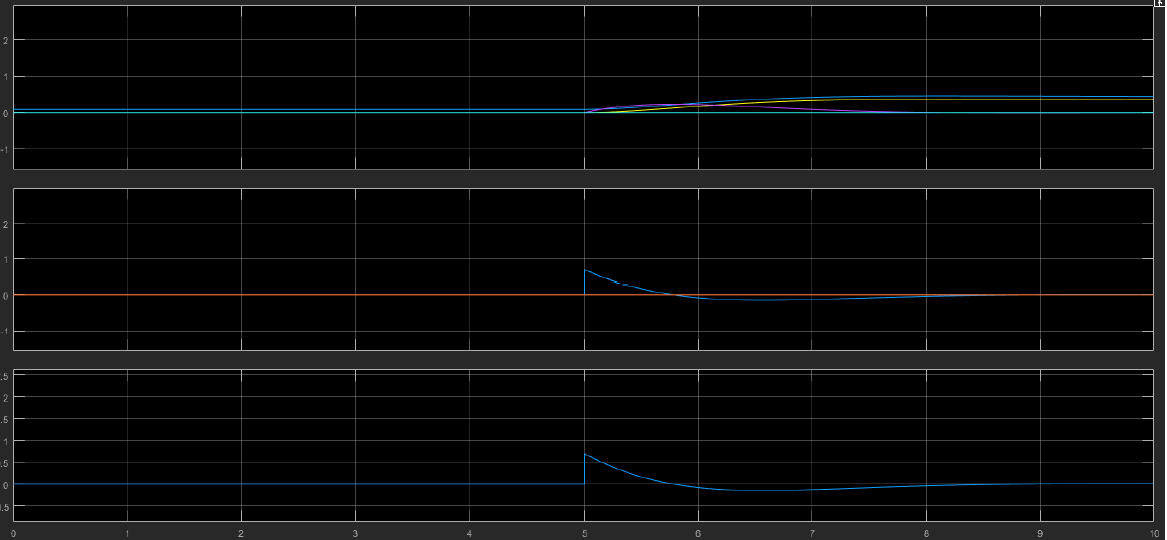
\includegraphics[width=0.9\textwidth]{S-Functions.png}
    \caption{Simulação S-Functions.}
    \label{fig:mesh3}
\end{figure}

\quad No gráfico da \textbf{Figura 3} temos a variação do $body$ $pitch$, em azul, e $body$ $yaw$, em vermelho. Nele também pode-se observar a resposta do sistemas à pertubações em sua inércia, onde se tem o assentamento como resposta das derivadas na ordenada nula. Da mesma forma, o gráfico superior representa o $body$ $pitch$ e $body$ $yaw$, de acordo com o avanço temporal.

\subsubsection{ode45}

\quad Utilizando o arquivo \emph{“NXTway\underline{\hspace{.1in}}figs.m”}, é obtido outra forma de visualização da \textbf{Figura 3}.

\begin{figure}[H] 
    \centering
    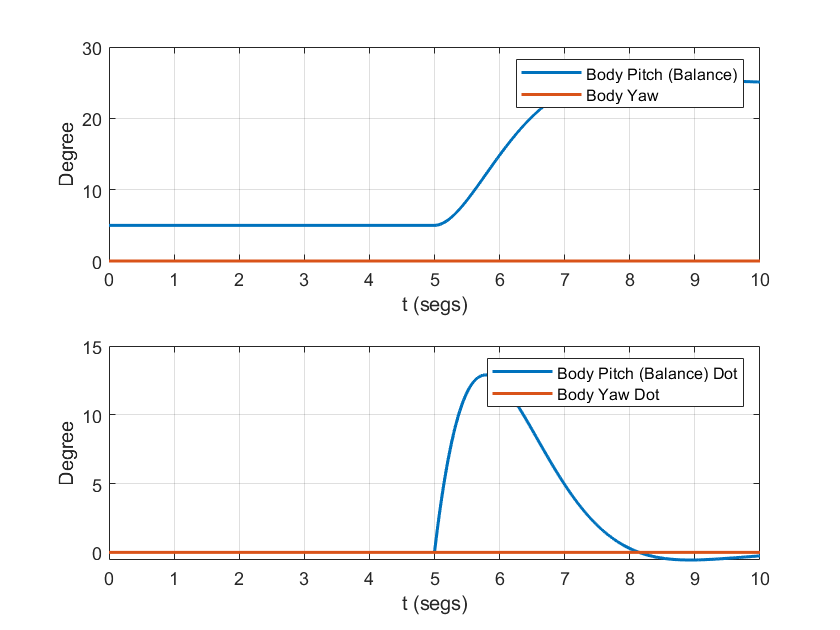
\includegraphics[width=0.9\textwidth]{FIGURA03.png}
    \caption{Simulação ode45.}
    \label{fig:mesh3}
\end{figure}

\quad Apesar representar o mesmo da \textbf{Figura 3}, nesta visualização temos as transições de \emph{body yaw Dot} de forma menos intensa. 

\subsubsection{Modelo Linear}

\quad Utilizando o algoritmo abaixo, modelo linear foi simulado, com apoio da ferramenta \textbf{ode45} do Matlab:

\begin{figure}[H] 
    \centering
    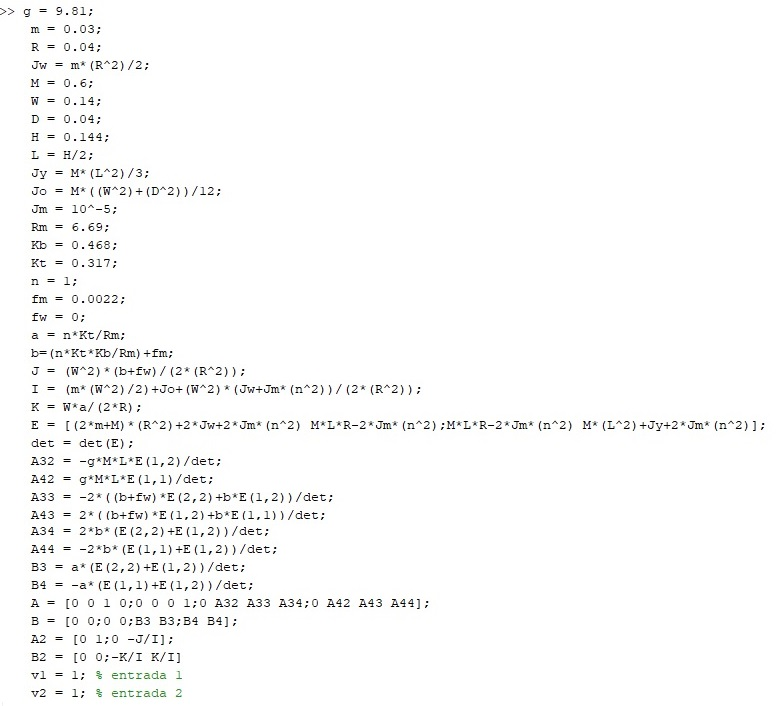
\includegraphics[width=1.2\textwidth]{matlab1.jpg}
    \label{fig:mesh6}
\end{figure}


\quad Para as entradas do sistema, $v_1$ e $v_2$, é valor unitário. Assim, é representado o sistema com a aplicação de um degrau unitário.Conforme o comando abaixo, são simuladas as características do \emph{body pitch}:

\begin{figure}[H] 
    \centering
    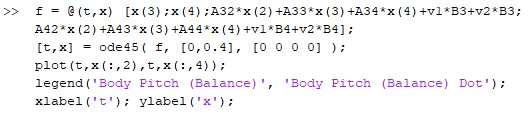
\includegraphics[width=1\textwidth]{matlab2.jpg}
    \label{fig:mesh6}
\end{figure}



\quad Foi necessário segmentar a variação temporal, a fim de  mantê-la próxima de zero. Uma vez que este modelo é compatível somente com as proximidades do ponto em que ocorreu a linearização, com um período amostral grande, o efeito esperado do sistema deixa de ser observado. Ao utilizar o algoritmo, obtemos o seguinte gráfico:

\begin{figure}[H] 
    \centering
    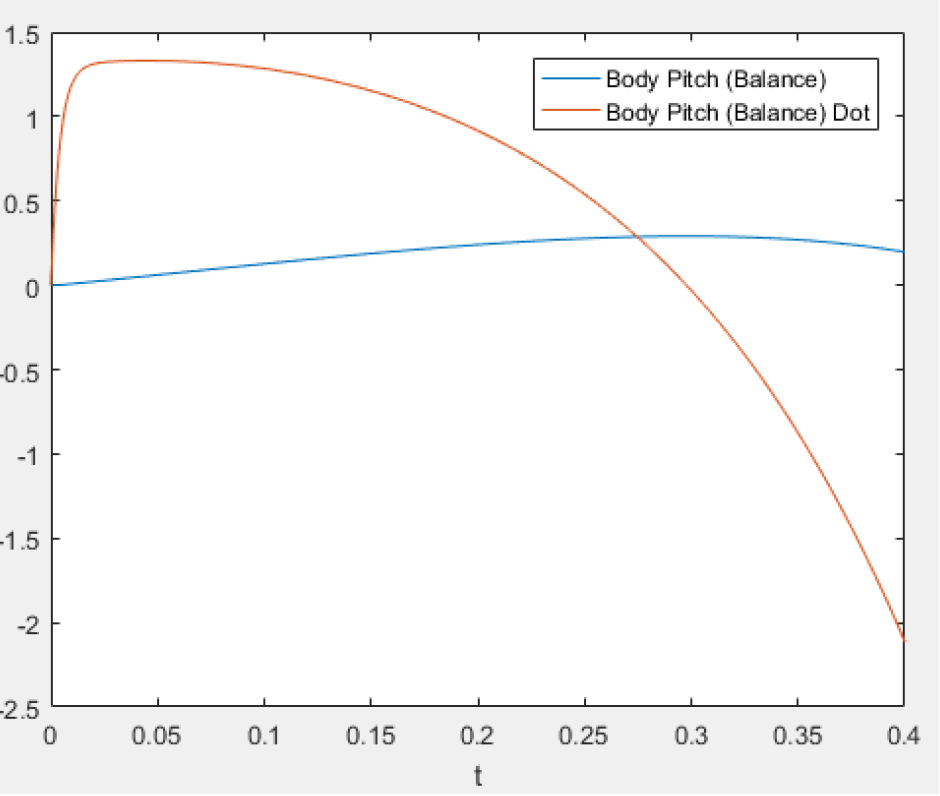
\includegraphics[width=0.9\textwidth]{FIGURA07.png}
    \caption{Modelo Linearizado Body Yaw.}
    \label{fig:mesh3}
\end{figure}

Por conseguinte, código seguinte retorna a resposta da variação do \emph{body yaw}:

\begin{figure}[H] 
    \centering
    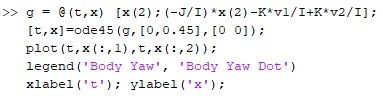
\includegraphics[width=0.7\textwidth]{matlab3.jpg}
    \label{fig:mesh3}
\end{figure}


\quad Obtemos o seguinte gráfico:

\begin{figure}[H] 
    \centering
    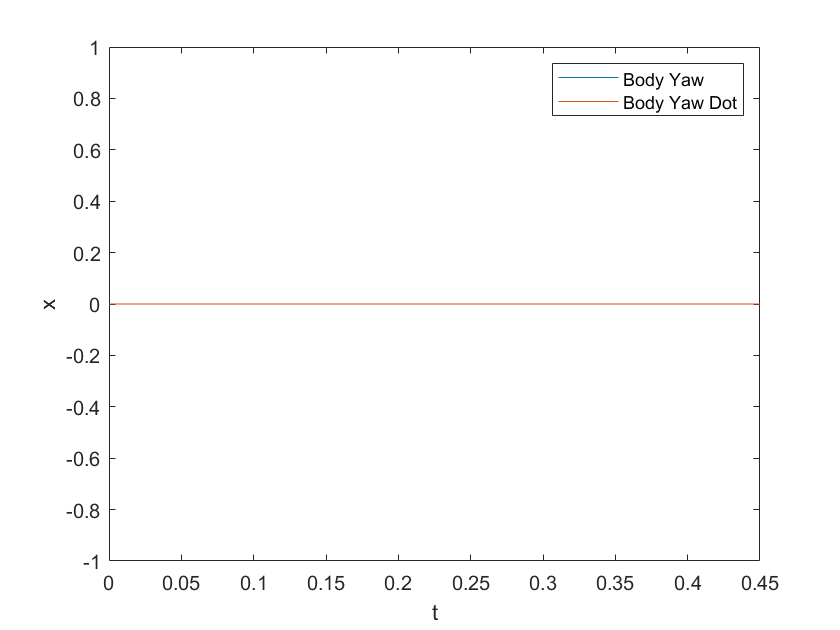
\includegraphics[width=0.9\textwidth]{FIGURA06.png}
    \caption{Modelo linearizado Body Yaw dot.}
    \label{fig:mesh3}
\end{figure}
\section{Discussão de Resultados}
\subsection{Análises}

\subsubsection{Variação do \emph{body yaw}}

\quad A partir da \textbf{Figura 4} é possível perceber como o sistema é não linear. No momento em que analisamos a
quebra do estado inercial do \emph{body yaw}, é possível observar uma trajetória de
curva, visualmente similar a uma representada por uma função de segundo
grau. Entretanto lidamos com um tempo de subida menor que o
tempo de descida, observável pela inclinação das curvas. Ainda, é possível ver
que, passado o tempo de resposta da perturbação, o sistema volta a operar em
um estado inerte, com variação aproximadamente nula do \emph{body yaw}.

\par De forma similar, \textbf{Figura 5}também
remete, visualmente, ao escopo de uma função de segundo grau. Suas
propriedades são similares ao da referência. Ainda, como mencionado
anteriormente, o período de amostragem foi curto, em decorrência da perda
de informações úteis, a longo prazo, de um modelo linearizado. Neste caso, é
possível ver este efeito, dado que, passado o tempo de resposta à perturbação,
o sistema não volta a um estado inerte na ordenada nula.

\par Unindo as informações, é possível concluir positivamente sobre a
compatibilidade entre o modelo não linearizado e o linearizado, mas somente
quando analisamos este em pontos próximos ao linearizado. 

\subsubsection{Variação do \emph{body yaw}}

\quad Ainda a partir \textbf{Figura 4} vemos que a
variação do \emph{body yaw}, se manteve constante, em valor nulo. O mesmo ocorreu
com a resposta indicada na \textbf{Figura 6}, o que indica compatibilidade entre ambos
os modelos, de forma satisfatória.

\subsection{Controle Realimentado}

\quad O sistema de controle é baseado em:

\begin{equation}
    u = -K_x + N_r
\end{equation}

Em que temos:

\begin{equation}
    {x_1}^T = \begin{bmatrix}
    \theta & \Psi & \phi & \dot{\theta} & \dot{\phi} 
    \end{bmatrix}
\end{equation}

\begin{equation}
    u^T = \begin{bmatrix}
    v_l & v_l
    \end{bmatrix}
\end{equation}

\begin{equation}
    N^T = \begin{bmatrix}
    -0.70771 & 0.0701\\
    \end{bmatrix}
\end{equation}

\begin{equation}
    K = \begin{bmatrix}
    - 0.0224 & -25.4867 & -0.7071 & -1.0362 & -2.2530 & -0.0076\\
    -0.0224 & -25.4867 & 0.7071 & -1.0362 & -2.2530 & 0.0076
    \end{bmatrix}
\end{equation}

\quad Ao manipular os códigos anteriores e adicionar novos parâmetros. Neste caso, foi selecionado valor unitário para 'r', a fim de ver as influências que a referência de comando do sistema tem. Em seguida, reajustando os parâmetros de $x_1$, de acordo com a realimentação proposta, encontramos a seguinte resposta para o \emph{body pitch}:

\begin{figure}[H] 
    \centering
    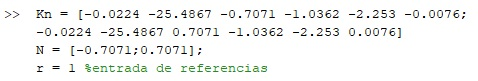
\includegraphics[width=0.8\textwidth]{matlab4.jpg}
    \label{fig:mesh3}
\end{figure}

\begin{figure}[H] 
    \centering
    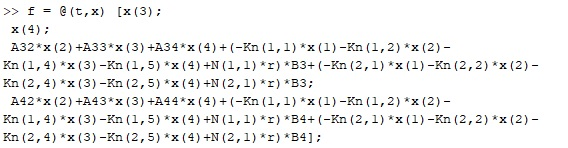
\includegraphics[width=0.8\textwidth]{matlab5.jpg}
    \label{fig:mesh3}
\end{figure}

\begin{figure}[H] 
    \centering
    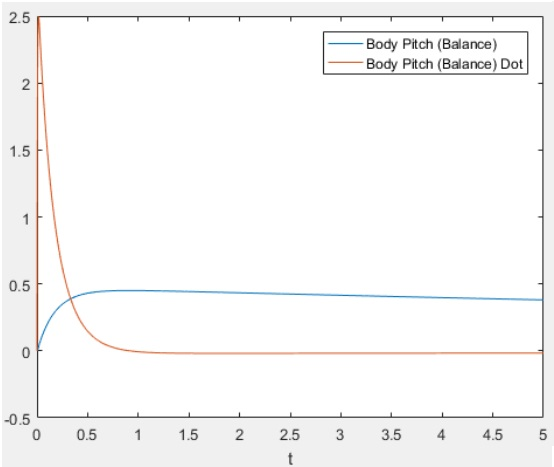
\includegraphics[width=0.7\textwidth]{pitch.jpg}
    \caption{body yaw Realimentado}
    \label{fig:mesh3}
\end{figure}

\quad Como observado, o gráfico plotado é parecido ao encontrado na \textbf{Figura 4}. Porém, diferentemente do que foi observado no modelo linearizado, este modelo atua como esperado em todos os pontos do período de análise, reagindo à pertubações, mas mantendo-se estável em estado de inércia.

\quad Com relação ao \emph{body yaw}, encontramos:

\begin{figure}[H] 
    \centering
    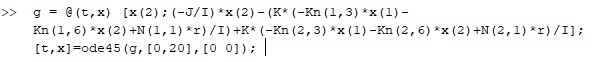
\includegraphics[width=1\textwidth]{matlab6.jpg}
    \label{fig:mesh3}
\end{figure}


\begin{figure}[H] 
    \centering
    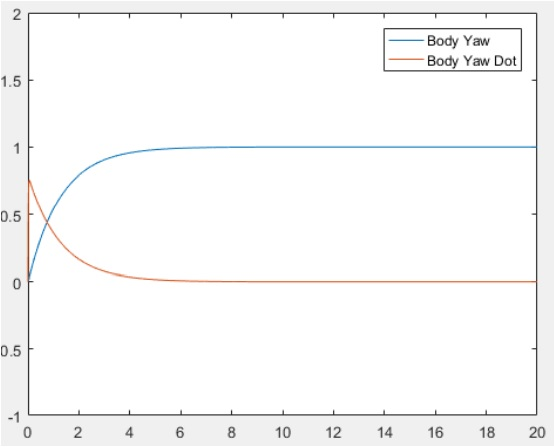
\includegraphics[width=0.7\textwidth]{fig4.jpg}
    \caption{body yaw Realimentado.}
    \label{fig:mesh3}
\end{figure}

\begin{figure}[H] 
    \centering
    \includegraphics[width=0.7\textwidth]{yaw.jpg}
    \caption{Body yaw Realimentado, r = 0}
    \label{fig:mesh3}
\end{figure}

\quad Neste gráfico é possível ver a influência que o fator 'r' possui sobre a movimentação do \emph{Segway}; o \emph{body yaw} do sistema estabiliza-se no valor indicado por 'r'. Ainda, como esperado, assim que o sistema alcança o equilíbrio, constante, a variação (\emph{body yaw} dot) tende a zero, assim como foi apresentado os modelos anteriores.

\quad Como exemplo de que este modelo mantém-se compatível com os demonstrados anteriormente, a figura 8 indica a resposta do \emph{\emph{body yaw}} quando 'r' é definido nulo.


\end{document}
